% --- Configuration ------------------------------------------------------
% add shortcut for github url of this chapter
\def \GITHUB {\GITHUBBASE/04_binaural_synthesis}
% add the fig folders
\graphicspath{%
{\PATH/\CHAPFOUR/fig4_01/}%
{\PATH/\CHAPFOUR/fig4_02/}%
{\PATH/\CHAPFOUR/fig4_03/}%
{\PATH/\CHAPFOUR/fig4_04/}%
{\PATH/\CHAPFOUR/fig4_05/}%
{\PATH/\CHAPFOUR/fig4_06/}%
{\PATH/\CHAPFOUR/fig4_07/}%
{\PATH/\CHAPFOUR/fig4_08/}%
{\PATH/\CHAPFOUR/fig4_09/}%
}


% --- Document -----------------------------------------------------------
\chapter{Binaural Synthesis and Experimental Setup}
\label{cha:binaural}

\firstthought{The auditory perception} of an acoustic event is largely triggered by the input
signals to the ear drums. Other influences like multi-modal interactions from the
visual or tactile senses have contributions to the auditory perception but
will be neglected here as a first approximation. Hence, it is possible to simulate any
acoustical event by synthesizing the corresponding signals at the ear
drum.\autocite{Moller1992} One
solution to achieve this is the application of binaural synthesis. For binaural
synthesis the transfer functions of an acoustic source 
to the two ears of the listener are measured in the desired environment.
Afterwards, any audio signal can be
convolved with the time signal corresponding to the transfer function and then played
back to the listener over headphones. If the headphones are considered as
an acoustically transparent system the signals of the ear drums of the listener
correspond to the ones from the acoustic source for which the transfer function was measured.
As this thesis is only interested in the investigation of sound field synthesis
methods without the influence of the reproduction room, an anechoic chamber is
chosen as environment. The transfer functions are then called
\emph{\acfp{HRTF}}.\footnote{To simplify the syntax
transfer functions measured in a room will also be called \acp{HRTF} in this
thesis and not binaural room impulse responses (BRTFs) as it is often the case
in the literature.}
%
\begin{figure}
    \centering
    \small
    \begin{tikzpicture}
        \draw (0,0)       node {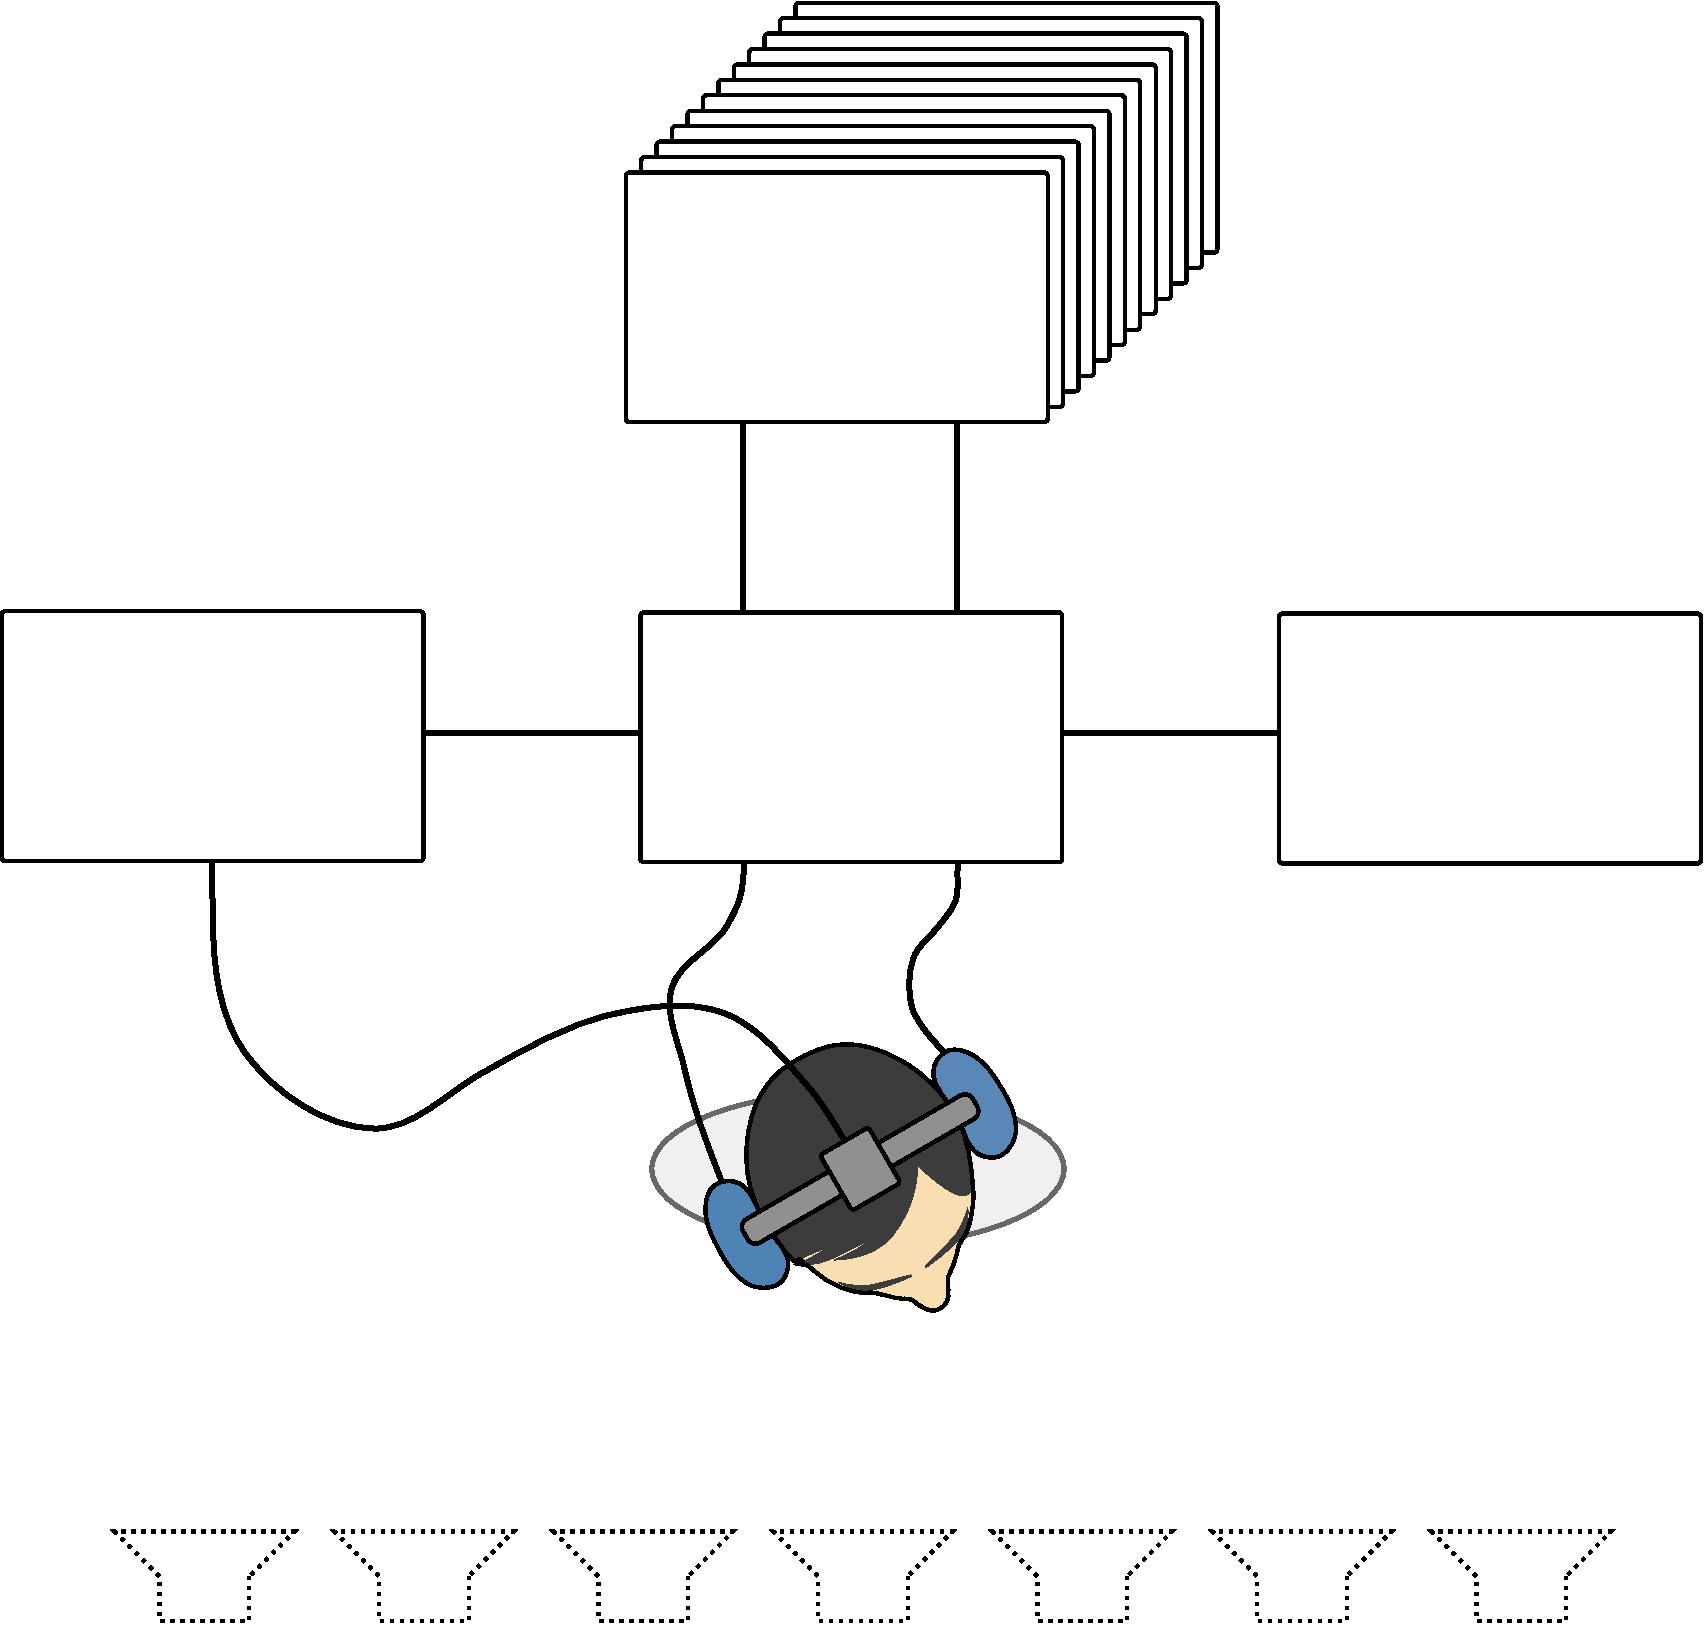
\includegraphics[width=.8\columnwidth]{dynamic_binaural_synthesis}};
        \draw (-0.06,2.9) node {\ac{HRTF}};
        \draw (-0.06,2.4) node {\scs\shortstack{for \\head orientation $\phi$}};
        \draw (0,0.7)     node {\acs{SSR}};
        \draw (0,0.1)     node {\scs\shortstack{convolution and \\ \ac{HRTF} switching}};
        \draw (-3.2,0.7)  node {\ft head tracker};
        \draw (-3.2,0.1)  node {\scs\shortstack{ head orientation $\phi$}};
        \draw (3.2,0.4)   node {\ft\shortstack{dry \\ audio material}};
        \draw (0,-4.5)    node {\ft simulated loudspeakers};
    \end{tikzpicture}
    \caption{Functional principle of dynamic binaural synthesis. The listener is
    wearing headphones and a head tracker. The audio material is convolved with
    the \ac{HRTF} that incorporates all simulated loudspeakers for the
    corresponding listener orientation.
    \reproduce{\GITHUB/fig4_01}}
    \label{fig:dynamic_binaural_synthesis}
\end{figure}


\newthought{One of the drawbacks} of static binaural synthesis is the assumption of a static
listener which can move neither head nor body. This can be overcome by measuring
transfer functions for different positions and head-orientations of the listener
and the usage of a head tracker system at reproduction time in order to switch
the transfer functions accordingly. The binaural synthesis is then termed dynamic
binaural synthesis or \ac{BRS}\autocite{Horbach1999a} -- compare
Fig.\,\ref{fig:dynamic_binaural_synthesis}.

A corresponding problem is the large number of measurements that are required.
Ideally, different positions and head-orientations for every single listener have to be
measured. In order to limit the number of measurement points,
non-individual transfer functions are often recorded with a dummy head that
mimics a common listener. Another restriction applied here is to limit the possible movements
of the listener
to head rotations in the horizontal plane only.
With such restrictions dynamic binaural synthesis is
already possible with 360 or less measurements in the horizontal plane, one per
degree.\sidenote[][-0.5cm]{\cite{Lindau2008}}

The approximation by non-individual transfer functions leads to a binaural
synthesis which cannot be considered as transparent.
Deviations in the magnitude of the transfer function may
be perceived as a change in timbre of the signal.\autocite{Takanen2012}
A mismatch in
the ear distance of the dummy head and the listener can lead to a slight
moving of the sound source with head movements of the
listener.\autocite{Algazi2001b}

The usage of a dummy head still implies a lot of measurements,
if not only head movements but different source directions are considered.
For all source directions a measurement with 360 head-orientations will sum up to
a measurement with 129\,600 points. This can be simplified by the assumption
that the difference between a
movement of the head relative to the torso or the movement of the head together
with the torso makes no perceptible difference in an anechoic
chamber.\autocite{Popko2013}

The usage of headphones for synthesizing the ear signals adds
another non-transparent component. Headphones have their own transfer function
which can be compensated only in a limited way due to the restrictions that exist
in filter design. Different labs have spent a large amount of time to come up
with systems that are transparent at least for some signals.
For instance, they built extraaural
headphones\autocite{Erbes2013} or developed techniques for fast individual \ac{HRTF}
measurements and individual headphone compensations.\autocite{Masiero2012}

Simplifying the prerequisites of this thesis, non-individual transfer functions
and commercially available headphones with a custom compensation filter  have
been used. In order to nevertheless get meaningful results, additional
experiments have been carried out to investigate the influence of the non-transparent binaural
synthesis on the different sound field synthesis feature addressed in this thesis
such as the localization and coloration of the created auditory events.

In the following section, the experimental setup common to all experiments of
this thesis is presented. Thereafter, experiments verifying the adequateness
of using
binaural synthesis to investigate different sound field synthesis issues are carried out.


%%%%%%%%%%%%%%%%%%%%%%%%%%%%%%%%%%%%%%%%%%%%%%%%%%%%%%%%%%%%%%%%%%%%%%%%%%%%%%%%
\section{Experimental Setup of Binaural Synthesis}
\label{sec:experimental_setup_of_binaural_synthesis}

%--%--%--%--%--%--%--%--%--%--%--%--%--%--%--%--%--%--%--%--%--%--%--%--%--%--%-
\subsection{Head-Related Transfer Function}
\label{sec:head-related-transfer-function}

\begin{marginfigure}
    \includegraphics[width=.98\columnwidth]{kemar_rar}
    \label{fig:kemar}
    \caption{Measurements with the artificial head in the anechoic chamber.
    \reproduce{\GITHUB/fig4_02}}
\end{marginfigure}

\urlnote{intpol\_ir.m}{\SFS/SFS_ir/intpol_ir.m}
\urlnote{get\_ir.m}{\SFS/SFS_ir/get_ir.m}
The \acp{HRTF} used for most of the binaural simulations
are part of a larger measurement conducted in the anechoic chamber of the
Technische Universität ({\small TU}) Berlin.\autocite[The \ac{HRTF} set is
\href{https://dev.qu.tu-berlin.de/projects/measurements/wiki/2010-11-kemar-anechoic}
{\color{link}{freely available}},
and is described in][]{Wierstorf2011a}\autocite[The author would like to
recommend the \href{https://sourceforge.net/projects/sofacoustics/}{\color{link}{Spatial Oriented
Audio File (\textsmaller{SOFA})}} format for the reader that is interested in \acp{HRTF}. It is a
joined effort between different labs to define a common file format for exchanging
\acp{HRTF} and other spatial oriented acoustical measurements. It is 
described in][]{Majdak2013}
The set used in this thesis for the experiments was measured in the horizontal
plane only. It has a distance of
$3$\,m between the loudspeaker (Genelec 8030A) and the dummy head ({\small
KEMAR}, type
45BA) and a resolution of $1\degree$.
For non-measured directions, \acp{HRTF} were calculated by linear interpolation.
For distances smaller or
larger than $3$\,m the \ac{HRTF} was adapted by delaying and weighting accordingly.
Loudspeaker arrays were created by a super-position of the \acp{HRTF}
corresponding to the single loudspeakers.


%--%--%--%--%--%--%--%--%--%--%--%--%--%--%--%--%--%--%--%--%--%--%--%--%--%--%-
\subsection{Apparatus}
\label{sec:apparatus}

Stimuli were digitally generated at a sampling rate of $44.1$\,kHz.
A computer was used to
generate impulse responses for the binaural synthesis. This could be an \ac{HRTF}
representing just one loudspeaker up to an array of loudspeakers driven by
signals calculated by one of the sound field synthesis methods,
depending on the experiment.
The convolution of the time signal of the \acp{HRTF} with
the audio signal was performed using the SoundScape
Renderer.\autocite[The \href{http://spatialaudio.net/ssr/}{\color{link}SoundScape
Renderer} is an open source software and is described in][]{Geier2008}
The audio signals were fed into the SoundScape Renderer via Pure
Data.\autocite[\href{http://puredata.info/}{\color{link}Pure Data} is an open
source software and first described in][]{Puckette1996}
The advantage of this setup is that Pure Data easily allows
to switch the output to another convolution instance of the SoundScape Renderer
including a pair of \ac{HRTF} representing another condition of the experiment. This
means that the listener can switch between different conditions within the
audio signal in contrast to the case where the audio signal starts playing from
the beginning for every switch.
The {\small PC} was equipped with an {\small RME HDSP MADI} card and for the
digital-to-analog conversion CreamWare A16 converters were used.
The listeners wore {\small AKG K601} headphones and a corresponding
headphone compensation filter was applied to the signals.
The head movements of the listeners were tracked by a Fastrak
Polhemus head tracker with a resolution of around $1\degree$, and the tracking
data were passed to the SoundScape Renderer.
The SoundScape Renderer was then switching the \acp{HRTF} for the dynamic binaural
synthesis, according to the
orientation of the listener given by the head tracker data.
Figure\,\ref{fig:dynamic_binaural_synthesis} illustrates the setup.

\newpage


%%%%%%%%%%%%%%%%%%%%%%%%%%%%%%%%%%%%%%%%%%%%%%%%%%%%%%%%%%%%%%%%%%%%%%%%%%%%%%%%
\section[Localization Experiments]{Verifying Binaural Synthesis for Localization
Experiments\autocite[Parts of this section are published
in][]{Wierstorf2012b,Wierstorf2013b}}
\label{sec:verifying_binaural_synthesis_for_localization_experiments}

The thesis aims to investigate localization in the audience area for different sound
field synthesis methods based on listening tests. To accomplish this, the ear signals
are simulated with dynamic binaural synthesis as outlined above. One requirement for this
kind of investigation is that the localization results will not be influenced by
the binaural synthesis. This will be verified in the following.

Experiments from the literature show that binaural synthesis has only
little influence on the results as long as its dynamic implementation is applied. In
this case, front-back confusions are avoided.
The localization error for real sources,
that is the absolute difference between the direction of a real
loudspeaker and direction of the auditory event lies between
$2\degree$ to $5\degree$.\autocite{Seeber2003a,Bronkhorst1995,Hess2004,Makous1990}
If individual \acp{HRTF} of the listeners were used, no difference between
localization of real and virtual speakers were found.
For non-individual \acp{HRTF} deviations
around $1\degree$ were found.\autocite{Seeber2003a}

One reason for the varying results for the localization performance in the
literature is the fact that localization experiments are critical
regarding the used pointing method. Due to the fact that the actual localization error
can be as small
as $1\degree$, the error of the pointing method has to be smaller than $1\degree$, which
cannot be achieved with all methods.\autocite{Majdak2008,Seeber2003a}

In order to test the influence of the pointing method and the dynamic binaural
synthesis with non-individual \acp{HRTF} on human localization a listening test
was conducted. Here, the localization of different loudspeakers
representing real sound sources and of the same sources simulated via dynamic
binaural synthesis were tested. If the localization results for the real sources
are comparable to the results from the literature, it indicates that the
accuracy of the pointing method is sufficient. If the localization results for
the simulated sources are equal to the ones of the real sources it proves that
the dynamic binaural synthesis has no influence on the localization results. If
both conditions are fulfilled the presented method is suitable for investigating the
localization in sound field synthesis.

First, the applied pointing method is introduced, followed by a description of
the experiment and the results.

%--%--%--%--%--%--%--%--%--%--%--%--%--%--%--%--%--%--%--%--%--%--%--%--%--%--%-
\subsection{Pointing Method}
\label{sec:pointing_method}

This thesis applies a pointing method that  Makous and
Middlebrooks\autocite{Makous1990} used in a similar way.
Here, the listener has to point with her head towards
the direction of the auditory event,
while the sound event is present.
This has the advantage that the listener is directly facing the source, a region
in which the minimum audible angle is the smallest.\autocite{Mills1958}
If the listener is pointing her nose in the direction of the source, an
estimation error of the sources at the side will occur, due to an interaction
with the human sensory-motor system. To overcome this, a visual pointer is
added, showing the
listener what her nose it pointing at.\autocite{Lewald2000}
To add such a visual pointer a small laser pointer was mounted onto the
headphones -- compare Fig.\,\ref{fig:apparatus}.

\begin{figure}[t]
    \begin{tikzpicture}
        \draw (-2.23,0)  node {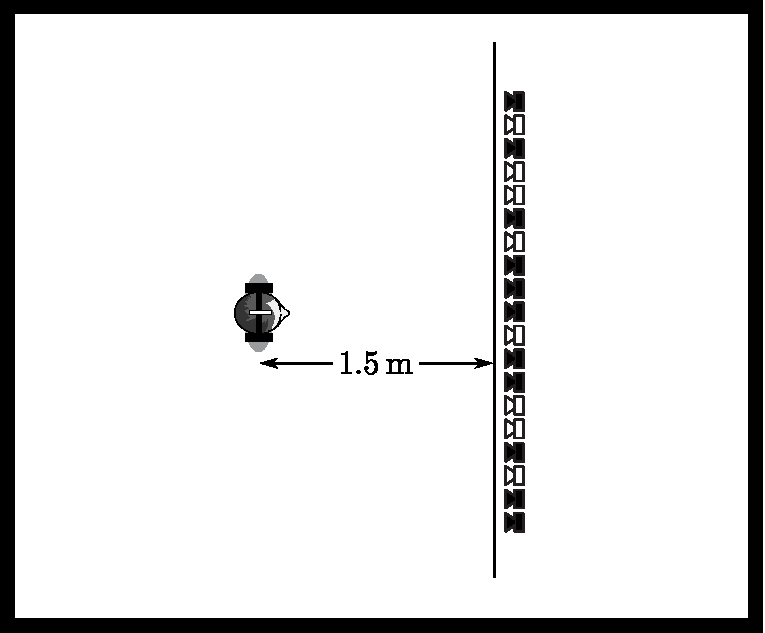
\includegraphics[width=.45\columnwidth]{apparatus}};
        \draw (3.2,0)    node {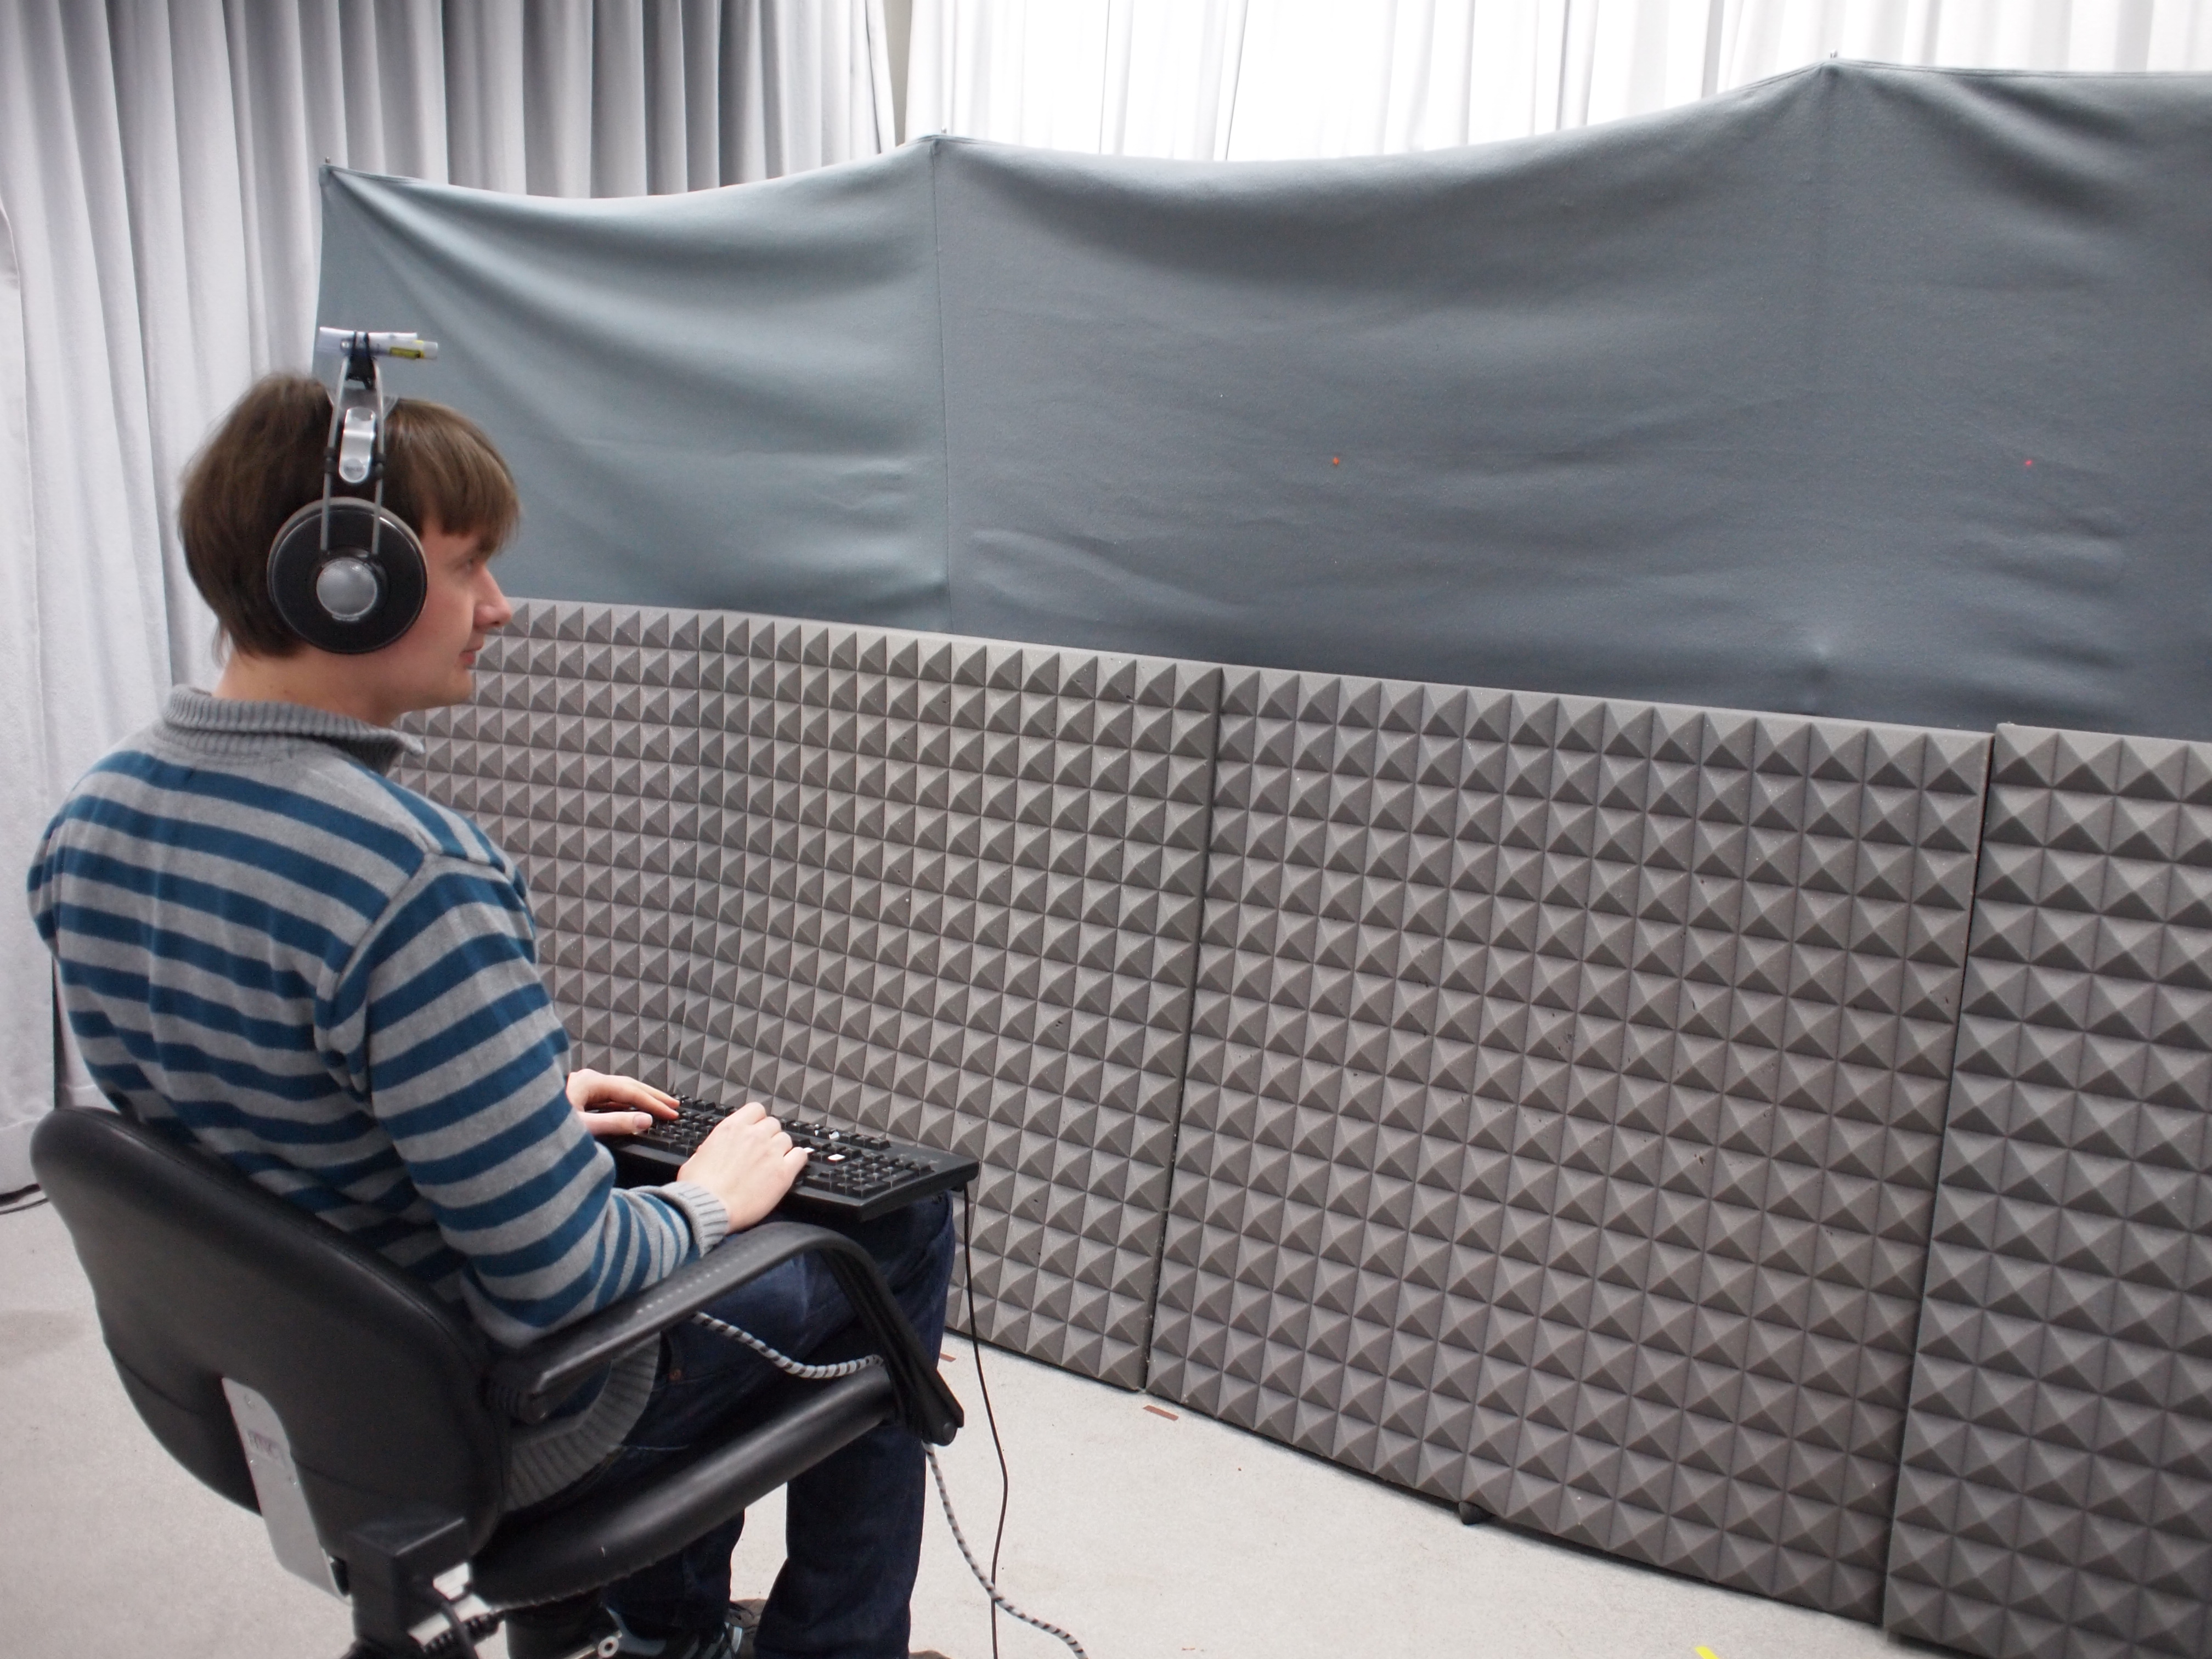
\includegraphics[width=.50\columnwidth]{procedure}};
        \draw (3.6,1.9)  node {\scs visual mark};
        \draw (5.27,1.9) node {\scs laser};
        \draw (3.6,1.7) -- (3.74,0.92);
        \draw (5.27,1.7) -- (5.41,0.92);
    \end{tikzpicture}
    \caption{Sketch of the apparatus in the listening room (left) and a listener
    during the experiment (right). Only the loudspeakers marked in black were
    used in the experiment. Note that the room was dark during
    the experiment.
    \reproduce{\GITHUB/fig4_03}}
    \label{fig:apparatus}
\end{figure}

%--%--%--%--%--%--%--%--%--%--%--%--%--%--%--%--%--%--%--%--%--%--%--%--%--%--%-
\subsection{Apparatus}
%
For the binaural synthesis the apparatus described in
Sec.\,\ref{sec:experimental_setup_of_binaural_synthesis} is applied.
In addition 19 Fostex {\small PM0.4}
loudspeakers were placed in an acoustically damped
listening room (room \emph{Calypso} in the Telefunken building of the {\small TU} Berlin).
The room has a volume of $83$\,m$^3$ and a reverberation time $RT_{60}$ of $0.17$\,s
at a frequency of $1$\,kHz.
The loudspeakers were arranged as a linear array with a spacing of $0.15$\,m
between them. Only the eleven loudspeakers highlighted in
Fig.\,\ref{fig:apparatus} were involved in the experiment.
The listener was positioned in a heavy chair,
$1.5$\,m in front of the
loudspeaker array, with an acoustically transparent curtain in between.
A sketch of the setup and a picture is shown in Fig.~\ref{fig:apparatus}.
The orientation and position of the listeners during the experiment was recorded
with the same head tracker that provides the data for the dynamic binaural synthesis.

%--%--%--%--%--%--%--%--%--%--%--%--%--%--%--%--%--%--%--%--%--%--%--%--%--%--%-
\subsection{Listeners}
%
Eleven adult listeners were recruited to conduct both parts of the experiment
-- aged 21 to 33 years.
Four of them had prior experiences with psychoacoustic testing.
The listeners were financially compensated for their effort.

%--%--%--%--%--%--%--%--%--%--%--%--%--%--%--%--%--%--%--%--%--%--%--%--%--%--%-
\subsection{Stimuli}
%
As audio material, Gaussian white noise pulses with a duration of $700$\,ms and
a
pause of $300$\,ms between them were applied. The single pulses were windowed
with a Hanning window of $20$\,ms length at the start and the end.
The signal was band-pass filtered with a fourth order butterworth filter with
its pass-band between $125$\,Hz and $20000$\,Hz.
The signal with a total length of $100$\,s was stored and played back in a loop
during the experiment. The single pulses of this signal were independent white noise
signals.
For the headphone reproduction the noise file was convolved with the time signal
of the corresponding \ac{HRTF}.

%--%--%--%--%--%--%--%--%--%--%--%--%--%--%--%--%--%--%--%--%--%--%--%--%--%--%-
\subsection{Procedure}
%
The listeners sat on a chair, wearing headphones with the mounted laser
pointer and had a keyboard on their knees -- see Fig.~\ref{fig:apparatus}.
They were instructed to use the point for pointing into the direction from where
they perceived the auditory event.
The test participants were informed that the vertical direction should be
ignored. After they made sure to point into the right direction, they were asked
to hit the enter key.
The listeners' head orientation was calculated as the mean over the
following $10$
values obtained from
the head tracker, which corresponds to a time of $90$\,ms.
After the key press, the next trial started instantaneously, which implied that
the listener always started the localization from the last position.
The listeners were instructed that they could turn their head if they were unsure
about the direction of the sound.

There were three conditions in the experiment, \emph{loudspeaker}, 
\emph{binaural synthesis}, and \emph{binaural synthesis with room reflections}.
In this thesis, only the first and second will be discussed. The full experiment is presented
in Wierstorf et al.\autocite{Wierstorf2012b}

For the first one, the noise pulses were
played through any of the eleven loudspeakers. For the other two conditions the sound
was played via headphones. Three different conditions and eleven
different loudspeakers led to 33 trials.
Every listener had to pass all 33 trials six
times. The first 33 trials were for training, thereafter a session with 66
trials and one with 99 trials was passed. The order of the
conditions and presented loudspeakers was randomized.
In average the listeners needed 15~minutes to complete the experiment
excluding the training.

At the beginning of each session, a calibration was carried out. First, the
loudspeaker at $0\degree$ was active, and the listener had to look into the
respective direction in order to calibrate the head tracker.
In a second step, the listener
was indicated to point towards a given visual mark on the curtain. The
second step formed a connection between the head tracker orientation and the
room. After the calibration, the room was darkened and the
experiment started.

%--%--%--%--%--%--%--%--%--%--%--%--%--%--%--%--%--%--%--%--%--%--%--%--%--%--%-
\subsection{Data Analysis}
%
The listener was able to turn her head, and move the head
in a translatory way. For the conditions employing
headphone reproduction, this had no influence on the results for the perceived
direction, because the dynamic binaural synthesis compensated only for the angle
of the head, not for its absolute position. Hence, the virtual source was moving with
the listener in case of translational movements.
For the loudspeaker condition, this is no
longer true, and the perceived angle between a loudspeaker and the head of
the listener is changing with possible translatory head movements.
To calculate the direction of the auditory event, the data was
compensated for these head movements, which were acquired by the head tracker,
by the following formula.
\begin{equation}
    \phi' = \tan^{-1}\left( [ (1.5-y) \tan\phi - x ] / 1.5 \right)
\end{equation} 
Here $\phi$ is the measured head orientation, $x,y$ are the measured 
coordinates of the head tracker, assuming that the origin of the coordinate
system is at the center of the chair, and $\phi'$ is the final value for the
direction of the auditory event.
In an additional step, the measured orientation of the head had to be connected
to the orientation of the listener within the room. This step is needed
because the orientation of the head tracker is not an absolute value and was
chosen anew in every session.
In practice, this was solved by compensating
the measured head orientation data with the position of a tiny visual mark on
the curtain. Its position in the current head tracker orientation coordinate
system was measured in the calibration step.

%% NOTE: I'm not sure if this was done for the data or not, because in the
%% current version of the analyzing script it is not the case.
%The main problem which had to be solved for the \ac{HRTF} conditions
%was the relative zero point of the head tracker. To compensate for this, we assumed
%that the localization was symmetrical to the left and the right.
%Then the zero point of the localization data is the mean value of all
%measured directions of the auditory event in one session.
%In order to avoid an overreaching of the \ac{HRTF}
%conditions this step was also done for the loudspeaker condition.

After the data calibration, the results from both sessions were pooled for every
listener and the mean and standard deviation were calculated. The average over all
listeners together with the confidence interval\autocite{Cumming2007} was then
calculated using these data.

%--%--%--%--%--%--%--%--%--%--%--%--%--%--%--%--%--%--%--%--%--%--%--%--%--%--%-
\subsection{Results}
\label{sec:results_binaural_localization}
%
\begin{figure}
    \small
    \centering
    \input{fig4_04/binaural_synthesis_localization}
    \caption{Difference between the direction of the auditory event and the
    sound event for loudspeakers and the binaural simulation of the
    loudspeakers. Average over all listeners together with the $95\%$ confidence
    interval is shown.
    \reproduce{\GITHUB/fig4_04}}
    \label{fig:binaural_synthesis_localization}
\end{figure}
%
\noindent One listener had a standard deviation that was twice as high as that of
the other listeners. The measurements from this listener
were excluded from the results.
Figure\,\ref{fig:binaural_synthesis_localization} shows the average over the listeners,
together with the $95\%$
confidence intervals.
The difference between the direction of the auditory event and the direction of
the sound event is shown.
It states that it never exceeds $5\degree$ for any condition and
loudspeaker, but a slight underestimation
of the loudspeakers at the sides can be observed for both conditions.
As another measure the mean of the standard deviations of the listeners was calculated.
The loudspeaker condition has an average standard deviation of 
$2.2\degree \pm 0.2\degree$. For the binaural synthesis  condition the standard
deviation is slightly higher at $3.8\degree \pm 0.3\degree$.

%--%--%--%--%--%--%--%--%--%--%--%--%--%--%--%--%--%--%--%--%--%--%--%--%--%--%-
\subsection{Discussion}
%
Exclusively considering the results for $-30\degree$ to $30\degree$ of the direction
of the sound event, the localization error for the loudspeakers
is around $1\degree$-$2\degree$ which is in agreement with the literature and
indicates that the resolution of the pointing method is sufficient. For sound
event positions closer to the side a slight undershoot of the direction of the
auditory event is visible. This means that the listener is not looking far enough
to the side. This effect is known from pointing methods without visible
feedback, which should be compensated for with the laser pointer giving visual
feedback. To overcome this problem, which is also prominent in the results for
the binaural synthesis condition, only sound events in the range from
$-30\degree$ to $30\degree$ will be investigated in further experiments.

The next question to answer is the influence of the binaural simulation on the
localization accuracy in comparison to the case of real loudspeakers. The
average localization error together with its confidence interval is $2.4\degree
\pm 0.3\degree$ for the loudspeaker condition and $2.0\degree \pm 0.4\degree$
for the binaural synthesis condition. This allows the conclusion that the
simulation of the loudspeakers by dynamic binaural synthesis has no influence on
the localization accuracy that can be achieved. That means binaural
simulations can be used to study localization for different loudspeaker setups
as they are needed for sound field synthesis.

Interestingly the average standard deviation is significant higher for
the binaural synthesis condition than for the loudspeaker condition. This
correlates with the finding that the listeners needed longer for answering in the case
of the binaural synthesis. The average time after the start of the stimulus and
the pressing of the answer key was $3.5$\,s $\pm 0.7$\,s for the loudspeaker
condition and $5.5$\,s $\pm 1.7$\,s in the case of the binaural simulation.
This indicates that even though the average localization accuracy is not affected by
the binaural simulation, it takes more effort for the listener to find the
position of the auditory event in the case of dynamic binaural synthesis.

%--%--%--%--%--%--%--%--%--%--%--%--%--%--%--%--%--%--%--%--%--%--%--%--%--%--%-
\subsection{Conclusion}
%
It was found that the accuracy of the applied pointing method is
sufficient as long as the sound event is not placed more than $\pm 30\degree$ to the
side of the listener. In addition, the binaural simulation of the loudspeakers
has a negligible influence on the localization accuracy of the test
participants. Only the time
and the certainty with which the listeners localize the sound is slightly
degraded.
It can be concluded that the dynamic binaural synthesis method is a proper tool
to investigate localization in \ac{SFS}.

\newpage

%%%%%%%%%%%%%%%%%%%%%%%%%%%%%%%%%%%%%%%%%%%%%%%%%%%%%%%%%%%%%%%%%%%%%%%%%%%%%%%%
\section[Simulation of Loudspeaker Arrays]{Verifying Binaural Synthesis for Simulation of Loudspeaker
Arrays\autocite[Parts of this section are published in][]{Wierstorf2012}}
\label{sec:verifying_binaural_synthesis_for_simulation_of_loudspeaker_arrays}
%
Up to here only the binaural simulation of a single loudspeaker was considered.
In order to investigate sound field synthesis methods, arrays of
loudspeakers are of interest that can have up to thousands of loudspeakers. To
handle such setups it is practically preferable if the complete loudspeaker
array can be
simulated by a \ac{HRTF} set measured only for one loudspeaker. In this section it
will be discussed how this can be achieved and what differences can be expected
in comparison to the case of having \acp{HRTF} for the whole loudspeaker array.

\urlnote{get\_ir.m}{\SFS/SFS\_ir/get\_ir.m}
\urlnote{intpol\_ir.m}{\SFS/SFS\_ir/intpol\_ir.m}
If a \ac{HRTF} set for a single loudspeaker is measured for placements of the
loudspeaker all around the dummy head, \ac{HRTF} sets for loudspeaker arrays can be
created by applying interpolation, extrapolation and superposition
to the \acp{HRTF} from the set of
the single loudspeaker. The straightforward solution is to apply a linear interpolation
and a time delay and amplitude weight for the extrapolation.

One of the differences of simulating the whole array with an \ac{HRTF} from a single
loudspeaker is the absence of the other loudspeakers during the \ac{HRTF} measurement.
These other loudspeakers -- if active -- can influence the impedance
of the measured one. In addition the body of the loudspeakers can change 
the magnitude of the transfer function by adding reflections.
Völk et al.\autocite{Volk2010c} have investigated both effects. The influence of
the impedance is negligible, but the change in magnitude of the transfer
function can reach $4$\,dB.

Another influencing factor is the loudspeaker's directivity.
In the case of an \ac{HRTF} measurement of a single loudspeaker and
a common setup, that
loudspeaker is always pointing towards the listener. Whereas in an \ac{HRTF}
measurement of a linear loudspeaker array, the single loudspeakers all are pointing in
the same direction and not towards the point where the listener is sitting. To
investigate the degree of difference due to the directivity, an \ac{HRTF} measurement
of a linear loudspeaker array was performed in an anechoic chamber.

%--%--%--%--%--%--%--%--%--%--%--%--%--%--%--%--%--%--%--%--%--%--%--%--%--%--%-
\subsection{Method}
%
\begin{marginfigure}
    \includegraphics[width=\columnwidth]{rar_kemar_array}
    \caption{\ac{HRTF} measurement of a loudspeaker array in the anechoic
    chamber of the \textsmaller{TU} Berlin.
    \reproduce{\GITHUB/fig4_05}}
    \label{fig:HRTF_measurement_array}
\end{marginfigure}
%
\acp{HRTF} of an loudspeaker array were measured in the anechoic chamber of
the {\small TU}
Berlin. The same dummy head and hardware as described in Wierstorf et
al.\autocite{Wierstorf2011a} was used for the recording. The loudspeaker array
itself consisted of 13 Fostex {\small PM0.4} loudspeakers placed with a distance of
$15$\,cm between them and a distance of $2$\,m between the center loudspeaker
and the dummy head. In order to get results for larger arrays, the 13
loudspeakers were moved to the right and the left whereby the last two
loudspeakers of the array were placed at the same positions as the
two last loudspeakers of the central array on both sides. This means from the center
array the signals of 11 loudspeakers were recorded and for the side arrays the
signals of 12 loudspeakers, each. This corresponds to the size
of the whole array of 35 loudspeakers or an array length of $5.1$\,m.

To investigate the influence of the directivity the same loudspeaker array was
simulated via binaural synthesis by applying inter- and extrapolation to the \ac{HRTF} of the
single loudspeaker placed directly in front of the dummy head. The setup is
illustrated in Fig.\,\ref{fig:array_directivity}. Afterwards, for every
loudspeaker of both arrays the corresponding \ac{HRTF} was convolved with a $1$\,s
long white noise signal and fed into an auditory filterbank realized by
gammatone filters with a distance of $1$\,ERB. The magnitude was calculated by
building the root mean square value in every frequency channel.
\urlnote{auditoryfilterbank.m}{\AMT/modelstages/auditoryfilterbank.m}

%--%--%--%--%--%--%--%--%--%--%--%--%--%--%--%--%--%--%--%--%--%--%--%--%--%--%-
\subsection{Results and Discussion}
%
\begin{figure}
    \small
    \centering
    \input{fig4_06/array_directivity}
    \caption{Difference between the magnitude of the simulated and real
    loudspeaker array dependent on the center frequency of the auditory
    filter bank.
    \reproduce{\GITHUB/fig4_06}}
    \label{fig:array_directivity}
\end{figure}
%
The difference of the output signals in each frequency band was calculated for
the loudspeaker arrays. Figure\,\ref{fig:array_directivity} presents the
results. It can be seen that for frequencies greater than $7$\,kHz the signal
from the measured loudspeaker array is getting extenuated compared to the
simulated loudspeaker array. This extenuation is getting larger for higher
frequencies.

The main difference between the
simulated and the measured array is the orientation of the loudspeakers.
The difference in magnitude for high frequencies can be explained by a
non-omnidirectional directivity pattern for high frequencies, which is the case
for most loudspeakers. 


%--%--%--%--%--%--%--%--%--%--%--%--%--%--%--%--%--%--%--%--%--%--%--%--%--%--%-
\subsection{Conclusion}
%
A binaural simulation of a loudspeaker array can be implemented in two ways. One way is
to build the desired loudspeaker array in the anechoic chamber and then measure
the \ac{HRTF} set. The other way is to measure the \ac{HRTF} for a single loudspeaker and
create the array by superposition and inter- and extrapolation of the \ac{HRTF} of the single
loudspeaker to come up with the same array.

Both results will be slightly different. If a loudspeaker array is measured in
an anechoic chamber the other loudspeakers add additional reflections which will
alter the transfer function of the measured one up to
$4$\,dB.\autocite{Volk2010c} The loudspeakers of a linear array are all pointing
towards one direction whereas in the case of the simulation by a single
loudspeaker the loudspeakers are always pointing towards the listener. The directivity
pattern of the loudspeakers will lead to differences in the transfer
functions. Those differences will not be present for a circular loudspeaker array.

For the investigation of sound field synthesis methods the differences are
negligible or could be an advantage. The case of the binaural simulation using a single
loudspeaker allows to build a virtual loudspeaker array that better fits the
assumption made in the theory, namely that the loudspeakers are monopoles and
have no directivity and no influence upon another.
Hence, in this thesis binaural simulations of loudspeaker arrays will be produced
with the \ac{HRTF} of a single loudspeaker.


%%%%%%%%%%%%%%%%%%%%%%%%%%%%%%%%%%%%%%%%%%%%%%%%%%%%%%%%%%%%%%%%%%%%%%%%%%%%%%%%
\section[Coloration Experiments]{Verifying Binaural Synthesis for Coloration Experiments}
\label{sec:verifying_binaural_synthesis_for_coloration_experiments}

The investigation of changes in timbre with binaural synthesis is possible
only to some extent. The biggest problem is, that the synthesis itself introduces
changes in timbre, which can only be compensated for to some degree by using
individual \acp{HRTF} and individual headphone compensations.\autocite[Compare for
example][]{Masiero2012}

That means that an investigation of absolute coloration judgements will not be
possible with binaural synthesis, because the measured coloration could be due to
the synthesis process itself or due to the system under investigation and there
is no way to distinguish between both cases. If the absolute coloration due to
the binaural synthesis could be limited, the differences in coloration between
different simulated systems could be investigated under the assumption that the
binaural synthesis has the same influence on coloration for all systems.

One promising result from the literature is the study by Olive et
al.\autocite{Olive2007} who found no difference in the preference ratings for
four different loudspeakers between the measurement with real loudspeakers and
their binaural simulations. They applied non-individual \acp{HRTF} and non-individual
headphone compensation filters.
This was further supported by a study presented in
Wittek\autocite[][Fig.\,8.4]{Wittek2007} that found the same amount of
intra-system coloration for a stereophonic setup realized by real or simulated
loudspeakers. The simulation was done via dynamic binaural synthesis.

In this section the amount of deviation of the amplitude spectrum due to
binaural synthesis will be quantified to some extent. In addition, it will be
shown that the deviation of the spectrum will be the same, independent on the
simulated system. This is accomplished by recording both the ear signals for
the binaural simulation and the ear signals for the reproduction with real
loudspeakers each by using a dummy head. To consider the fact of
non-individual \acp{HRTF} recording is done with a different dummy head than the
measurement of the \acp{HRTF} that are used for the binaural synthesis.

%--%--%--%--%--%--%--%--%--%--%--%--%--%--%--%--%--%--%--%--%--%--%--%--%--%--%-
\subsection{Method}
%
\begin{marginfigure}
    \includegraphics[width=\columnwidth]{fabian}
    \caption{Recording of \acp{HRTF} with {\ft FABIAN} in room \emph{Pinta}. Note that this
    picture is from a recording session where {\ft FABIAN} was placed out of the center
    and did not wear headphones.
    \reproduce{\GITHUB/fig4_07}}
    \label{fig:pinta_recordings_setup}
\end{marginfigure}
%
\begin{marginfigure}
    \includegraphics[width=\columnwidth]{pinta_kemar}
    \caption{Recording of the ear signals for binaural synthesis and real loudspeakers in
    room \emph{Pinta}.
    \reproduce{\GITHUB/fig4_08}}
    \label{fig:pinta_recordings_setup}
\end{marginfigure}
%
In room \emph{Pinta} in the Telefunken building of {\small TU} Berlin a circular
loudspeaker array with 56 loudspeakers is installed. The room has a volume of
$54$\,m$^3$ and is acoustically damped with a reverberation time $RT_{60}$ of 
$0.81$\,s at a frequency of $1$\,kHz.
For all installed loudspeakers, \acp{HRTF} were measured with the {\small FABIAN} dummy
head\autocite[The measurements were performed by Alexander Lindau, the used
dummy head is described in][]{Lindau2007a}.
The dummy head was wearing {\small AKG K601} headphones
during the measurement. Wearing of open headphones during the measurement
is often done in \ac{HRTF} measurements for binaural
simulations. It allows the direct comparison of a reproduction by the real
or binaurally simulated loudspeaker by a listener without the need to remove the
headphone from her head in the experiment.\autocite[An example of 
verifying binaural synthesis is presented in][]{Lindau2012}

For the measurement the {\small KEMAR} dummy head was placed at the same
position in the center of the loudspeaker array in \emph{Pinta} as {\small
FABIAN} have been placed. Again open
{\small AKG K601} headphones were placed on its head. In this way,
the dummy head was able to
record sound coming from the loudspeakers going through the open headphones.
The \acp{HRTF} measured with {\small FABIAN} as described above were
used for a binaural simulation
which was then recorded by the {\small KEMAR} dummy head, too.

Four different conditions were compared. For the condition
\emph{mono} a single loudspeaker was active. The other three conditions involved
all the synthesis of a point source placed $1$\,m behind the array applying a
circular loudspeaker array with $14$, $28$, or $56$ loudspeakers and \ac{WFS}.
Note that
this corresponded to $4$, $9$, or $17$ active loudspeakers due to the secondary
source selection -- compare \eqref{eq:w_ps}.

For all four loudspeaker configurations the source was placed in the front, left,
right, or back of the dummy head, leading altogether to 16 different conditions.
The source consisted of a continuous white noise signal, that was
recorded for $24$\,s for every condition and position.


%--%--%--%--%--%--%--%--%--%--%--%--%--%--%--%--%--%--%--%--%--%--%--%--%--%--%-
\subsection{Results and Discussion}
%
\begin{figure}
    \small
    \centering
    \input{fig4_09/pinta_recordings}
    \caption{Differences in magnitude between real loudspeaker setups and their binaural simulation.
    A single loudspeaker (mono) or a circular loudspeaker array driven by
    \ac{WFS}
    was applied to synthesize a point source in the front, left, right, or back
    of the listener.
    \reproduce{\GITHUB/fig4_09}}
    \label{fig:pinta_recordings}
\end{figure}
%
Figure\,\ref{fig:pinta_recordings} shows the differences in magnitude between
the real loudspeakers and their binaural simulations for each condition.
The magnitude was calculated by processing the recorded noise signal with an
auditory filterbank and calculating the root mean square of the signal per band.
Afterwards, the
magnitude of the binaurally simulated loudspeakers was subtracted from the
magnitude of the real loudspeakers.
\urlnote{auditoryfilterbank.m}{\AMT/modelstages/auditoryfilterbank.m}

For all four positions, the deviations in magnitude are within $\pm5$\,dB up to
$5$\,kHz. For higher frequencies larger dips and peaks are visible going up to a
difference in magnitude of $15$\,dB for the single loudspeaker in the back.
The degree of deviation is not dependent on the condition type, and there is no
systematic change in deviation visible due to the number of used loudspeakers.
The only exception is the magnitude of the single loudspeaker for a frequency
around $15$\,kHz. At this frequency the deviation between the real and simulated
loudspeaker is stronger for all non-frontal source positions
than it is for all \ac{WFS} conditions.

The measurements showed that the deviation is independent of the number of
loudspeakers in the case of \ac{WFS}. The deviation between all \ac{WFS}
systems and the monaural source for some source positions at high frequencies
is still an open question and could not be solved with the conducted
experiments.

%--%--%--%--%--%--%--%--%--%--%--%--%--%--%--%--%--%--%--%--%--%--%--%--%--%--%-
\subsection{Conclusion}
%
In this thesis, experiments to quantify the coloration in sound field synthesis
methods were carried out. In order to investigate the usage of
non-individual \acp{HRTF} and a non-individual headphone compensation, dummy head
recordings were carried out. The fact of non-individual \acp{HRTF} was considered
by using two different dummy heads for the recording of the \acp{HRTF} that were used
for the binaural simulation and for the recording of the simulated results.

The results show that deviations up to $5$\,dB are present for frequency
channels below $5$\,kHz. For higher frequencies the deviation in magnitude
between a simulated and a real loudspeaker can be up to $15$\,dB.
Further, the measurements underlines the view that the offset in magnitude is a
linear process and it is independent of the number of simulated loudspeakers.
This assumption is necessary to compare different loudspeaker setups to each
other in a coloration experiment.

These results in combination with similarly supportive conclusions
from the literature are the
basis for applying the binaural synthesis to investigating coloration in
\ac{WFS} as described in Sec.\,\ref{sec:timbral_fidelity}.
